\documentclass{scrartcl}

\usepackage{amssymb}
\usepackage{amsmath}
\usepackage{tikz}
\usetikzlibrary{decorations.pathreplacing}	%for brackets (fig. 5)

%via Gorton, G. \& Metrick, A. (2010). ``Regulating the Shadow Banking System.'' \textit{Brookings Papers on Economic Activity}, pp. 261-97. [fig. 1,2,5]
%Retrieved from \url{https://www.brookings.edu/wp-content/uploads/2010/09/2010b_bpea_gorton.pdf}

\begin{document}
	
	%\begin{figure}
	%	\centering
	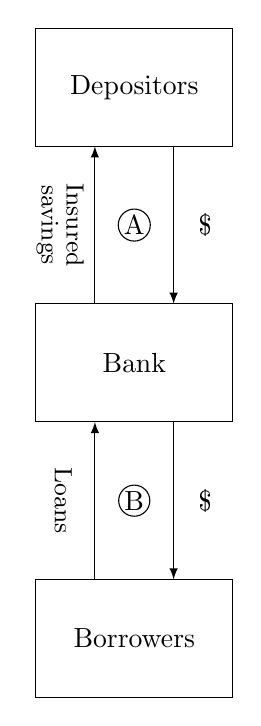
\begin{tikzpicture}
	\draw (0,3.5) rectangle (2.5,5);
	\node at (1.25,4.25) {Depositors};
		\node[circle,inner sep=0.5pt,draw] at (1.25,2.5) {A};
		\draw[->,>=latex] (0.75,1.5)--(0.75,3.5);
		\draw[->,>=latex] (1.75,3.5)--(1.75,1.5);
	\node at (0.5,2.5) {\rotatebox{270}{\small Insured}};
	\node at (.15,2.5) {\rotatebox{270}{\small savings}};
	\node at (2.15,2.5) {\$};
	%
	\draw (0,0) rectangle (2.5,1.5);
	\node at (1.25,0.75) {Bank};
	%
	\draw (0,-3.5) rectangle (2.5,-2);
	\node at (1.25,-2.75) {Borrowers};
		\node[circle,inner sep=0.5pt,draw] at (1.25,-1) {B};
		\draw[->,>=latex] (0.75,-2)--(0.75,0);
		\draw[->,>=latex] (1.75,0)--(1.75,-2);
	\node at (0.35,-1) {\rotatebox{270}{\small Loans}};
	\node at (2.15,-1) {\$};
	\end{tikzpicture}
	%	\caption{Traditional On-Balance-Sheet Intermediation}
	%\end{figure}
	%
	%
	\hspace{3cm}
	%
	%
	%\begin{figure}
	%	\centering
	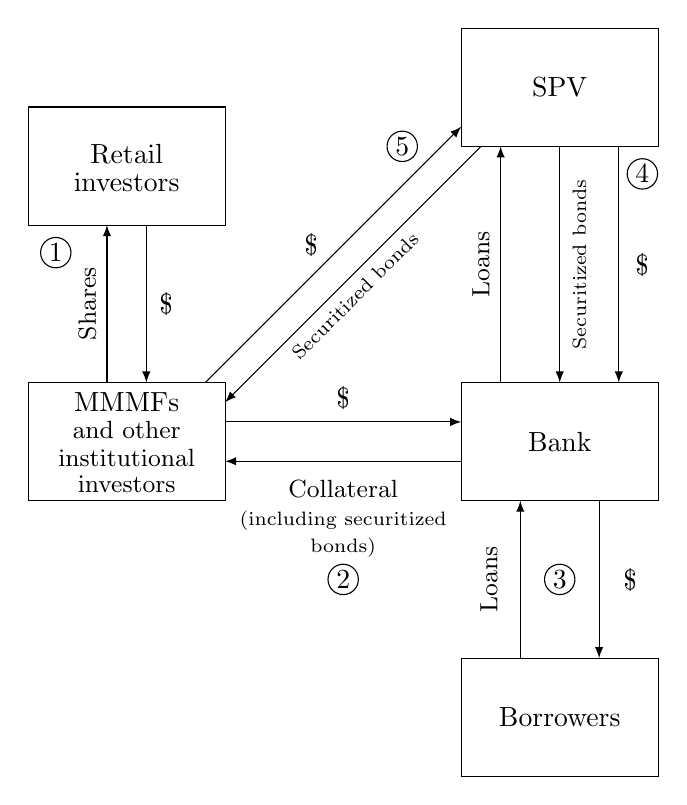
\begin{tikzpicture}
	\draw (0,4.5) rectangle (2.5,6);
	\node at (1.25,5.25) {SPV};
	\node at (1.5,3) {\rotatebox{90}{\scriptsize Securitized bonds}};
		\draw[->,>=latex] (0.5,1.5)--(0.5,4.5);
		\draw[->,>=latex] (1.25,4.5)--(1.25,1.5);
		\draw[->,>=latex] (2.0,4.5)--(2.0,1.5);
	\node at (0.25,3) {\rotatebox{90}{\small Loans}};
	\node at (2.3,3) {\$};
	\node[circle,inner sep=1pt,draw] at (2.3,4.15) {4};
	%
	\draw (-5.5,3.5) rectangle (-3,5);
	\node at (-4.25,4.40) {Retail};
	\node at (-4.25,4.05) {investors};
		\draw[->,>=latex] (-4.5,1.5)--(-4.5,3.5);
		\draw[->,>=latex] (-4,3.5)--(-4,1.5);
	\node at (-4.75,2.5) {\rotatebox{90}{\small Shares}};
	\node at (-3.75,2.5) {\$};
	\node[circle,inner sep=1pt,draw] at (-5.15,3.15) {1};
	%
	\draw (-5.5,0) rectangle (-3,1.5);
	\node at (-4.25,1.25) {MMMFs};
	\node at (-4.25,0.90) {\small and other};
	\node at (-4.25,0.55) {\small institutional};
	\node at (-4.25,0.21) {\small investors};
		\draw[->,>=latex] (-3.25,1.5)--(0,4.75);
		\draw[->,>=latex] (0.25,4.5)--(-3,1.25);
		\node at (-1.9,3.25) {\$};
		\node at (-1.35,2.6) {\rotatebox{45}{\scriptsize Securitized bonds}};
		%\node at (-1.35,2.5) {\rotatebox{45}{\small Securitized bonds}};		%too big
		\node[circle,inner sep=1pt,draw] at (-0.75,4.5) {5};
	%
	\draw (0,0) rectangle (2.5,1.5);
	\node at (1.25,0.75) {Bank};
		\draw[->,>=latex] (-3,1)--(0,1);
		\draw[->,>=latex] (0,0.5)--(-3,0.5);
	\node at (-1.5,1.3) {\$};
	\node at (-1.5,0.15) {\small Collateral};
	\node at (-1.5,-.25) {\scriptsize (including securitized};
	\node at (-1.5,-.60) {\scriptsize bonds)};
	\node[circle,inner sep=1pt,draw] at (-1.5,-1) {2};
	%
	\draw (0,-3.5) rectangle (2.5,-2);
	\node at (1.25,-2.75) {Borrowers};
		\node[circle,inner sep=1pt,draw] at (1.25,-1) {3};
		\draw[->,>=latex] (0.75,-2)--(0.75,0);
		\draw[->,>=latex] (1.75,0)--(1.75,-2);
	\node at (0.35,-1) {\rotatebox{90}{\small Loans}};
	\node at (2.15,-1) {\$};
	\end{tikzpicture}
	%	\caption{Off-Balance-Sheet Intermediation in the Shadow Banking System}
	%\end{figure}
	
	
	\vspace{2.5cm}
	
	
	%\begin{figure}
	%	\centering
	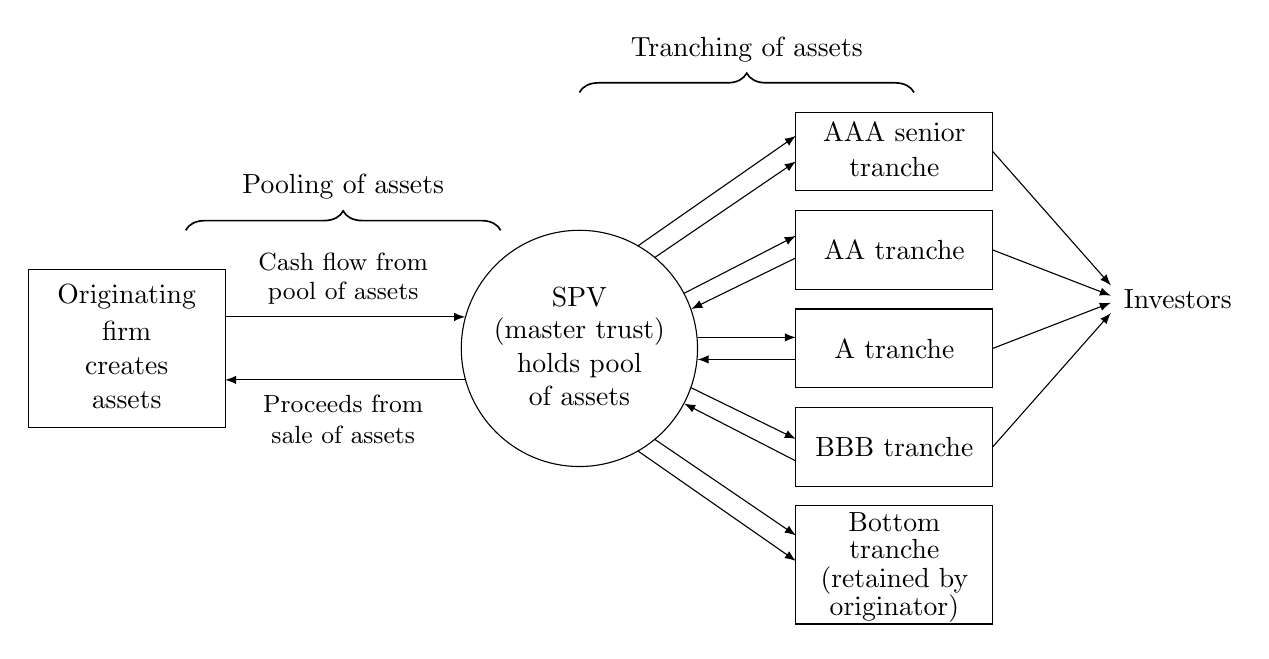
\begin{tikzpicture}
	%braces
	\node at (-3,2.05) {Pooling of assets};
	\draw[decorate,decoration={brace,amplitude=7pt},semithick] (-5,1.5)--(-1,1.5);
	%
	\node at (2.125,3.8) {Tranching of assets};
	\draw[decorate,decoration={brace,amplitude=7pt},semithick] (0,3.25)--(4.25,3.25);
	
	%box & circle
	\draw (-7,-1) rectangle (-4.5,1);
	\node at (-5.75,0.65) {Originating};
	\node at (-5.75,0.22) {firm};
	\node at (-5.75,-.22) {creates};
	\node at (-5.75,-.65) {assets};
	%
	\node at (-3,1.1) {\small Cash flow from};
	\node at (-3,0.7) {\small pool of assets};
	\draw[->,>=latex] (-4.5,0.4)--(-1.45,0.4);
	\draw[->,>=latex] (-1.45,-.4)--(-4.5,-.4);
	\node at (-3,-.7) {\small Proceeds from};
	\node at (-3,-1.1){\small sale of assets};
	%
	\draw (0,0) circle (1.5cm);
	\node at (0,0.65) {SPV};
	\node at (0,0.22) {(master trust)};
	\node at (0,-.22) {holds pool};
	\node at (0,-.60) {of assets};
	
	%arrows
	\draw[->,>=latex] (0.74,1.30)--(2.75,2.7);
	\draw[->,>=latex] (0.95,1.15)--(2.75,2.375);
	%
	\draw[->,>=latex] (1.33,0.7)--(2.75,1.43);
	\draw[->,>=latex] (2.75,1.15)--(1.42,0.5);
	%
	\draw[->,>=latex] (1.5,0.14)--(2.75,0.14);
	\draw[->,>=latex] (2.75,-.14)--(1.5,-.14);
	%
	\draw[->,>=latex] (1.42,-0.5)--(2.75,-1.15);
	\draw[->,>=latex] (2.75,-1.43)--(1.33,-0.7);
	%
	\draw[->,>=latex] (0.95,-1.15)--(2.75,-2.375);
	\draw[->,>=latex] (0.74,-1.30)--(2.75,-2.7);
	
	%tranches
	\draw (2.75,2) rectangle (5.25,3);
		\node at (4,2.75) {AAA senior};
		\node at (4,2.30) {tranche};
	\draw (2.75,0.75) rectangle (5.25,1.75);
		\node at (4,1.25) {AA tranche};
	\draw (2.75,-0.5) rectangle (5.25,0.5);
		\node at (4,0) {A tranche};
	\draw (2.75,-1.75) rectangle (5.25,-0.75);
		\node at (4,-1.25) {BBB tranche};
	\draw (2.75,-2) rectangle (5.25,-3.5);
		\node at (4,-2.20) {Bottom};
		\node at (4,-2.55) {tranche};
		\node at (4,-2.95) {(retained by};
		\node at (4,-3.30) {originator)};
	
	%rightmost arrows
	\draw[->,>=latex] (5.25,2.50)--(6.75,0.8);
	\draw[->,>=latex] (5.25,1.25)--(6.75,0.67);
	\draw[->,>=latex] (5.25,0)--(6.75,0.58);
	\draw[->,>=latex] (5.25,-1.25)--(6.75,0.45);
	\node at (7.6,0.625) {Investors};
	\end{tikzpicture}
	%	\caption{The Securitization Process}
	%\end{figure}
	
\end{document}